\chapter{Axions in Cosmology}


With the advent of precision cosmology in the 21st century, particle physicists can use the entire universe as a laboratory for ever more sensitive experiments.
Depending on the strength and variety of their interactions with other matter, axions may have significant implications for the evolution of the universe and of astrophysical structures, leaving behind detectable signatures.
Of special interest is the axion's promise as a dark matter candidate.
This section is a review of the current status of the axion in cosmology; its astrophysical predictions and observational constraints.
Primary sources are Cadamuro, Hannestad \etal., \cite[{}2011]{Cadamuro_2011}; Marsh \cite[{}2016]{Marsh_2016}; and Irastorza and Redondo \cite[{}2018]{Irastorza_2018}; along with sections of the Particle Data Group's \emph{Review of Particle Physics} \cite[{}2020]{ParticleDataGroup-review-2020}.






\section{The Standard Cosmological Picture}

Many cosmological tests of axion-like particles involve predicting relative particle abundances in the universe at various epochs, such as the baryon-to-photon or neutrino-to-photon ratios.
Such arguments begin with a minimal `thermodynamical' model of the universe as a homogeneous, isotropic, expanding background upon which different particle species exist in uniform thermal equilibrium.
The universe's macrostate is characterised by each species' abundance and energy distribution, and is characterised by a cosmological temperature, $T$, quantifying average energy density.
Interactions and processes between species, which at any time may depend on present particle abundances and energies, define differential relations which can be solved to determine the abundance of each species at any point in the universe's evolution.
In general, this is expressed by the \emph{Boltzmann transport equation}, describing the statistical behaviour of a thermodynamic system out of equilibrium. \note{Need to cite?}


\begin{figure}[b!]
\begin{aside}[Terminology from cosmology]
\begin{itemize}[leftmargin=0.75em]\setlength\itemsep{0.25ex}
	\item \emph{thermalisation}
---	the process of a particle species reaching thermal equilibrium (i.e., uniform energy and abundance) over cosmological scales, mitigated by energy-diffusing self-interactions or processes with other species.
	\item \emph{freeze-out}
---	the point beyond which the rates of thermalising processes become negligible due to cooling cosmological temperature or accelerating cosmic expansion. Freeze-out results in persistent non-equilibrium distributions of a particle species, analogous to a change of phase from a gas to a cooler condensate.
% Since the universe cools as it expands, freeze-out may be viewed as a species' change of phase from a gas to a cooler condensate.
\end{itemize}
\end{aside}
\end{figure}

The harsh assumptions of isotropy and homogeneity specify a spacetime with a Friedmann--Lemaître--Robertson--Walker (FLRW) metric,
\begin{align}
	% \ts g = -c^2 \ts\dd t\otimes\ts\dd t + a(t)^2\qty(η_{ij}\,\ts\dd x^i\otimes\ts\dd x^j)
	\ts g = -c^2 \ts\dd t^2 + a(t)^2\qty(\frac{\ts\dd r^2}{1 - kr^2} + r^2 \ts Θ)
\end{align}
where $k \in \qty{+1, 0, -1}$ reflects the type of spatial curvature, $\ts Θ = \ts\dd θ^2 + \sinθ\,\ts\dd φ^2$ is the metric of the unit sphere, and $\ts\dd x^2 \equiv \ts\dd x\otimes\ts\dd x$.
Standard cosmological models are spatially flat with $k = 0$.
The scale factor $a(t)$ describes the cosmological evolution of the universe and defines the \emph{Hubble parameter,} $H \coloneqq \dot{a}/a$, or cosmic expansion rate.
The equations of general relativity determine $a(t)$ uniquely in terms of the mass--energy content of the universe.

If the rate $Γ$ of a particle interaction is large (corresponding to large probability per unit spacetime volume for the interaction to occur), then it will provide a mechanism for thermalisation of the species involved---or in the case of production and decay processes, will drive the species to abundance or extinction. 
If the rate is smaller than the rate of cosmic expansion, $Γ \ll H$, then the interaction or process will freeze-out and become negligible.
Freeze-out may also result from the cosmological temperature $T$ being lower than a processes' threshold energy.
If a species' most dominant interactions freeze-out, then it becomes thermally isolated from other matter and its abundance remains fixed.








\section{Axion Interactions and Processes}

Axions spontaneously decay into photons via the axion-photon vertex at a well-known rate of
\begin{align}
	Γ_{a\to 2γ} = \frac{g_{aγγ}^2m_a^3}{64π} \approx 10^{-24}\,\si{\per\second}\qty(\frac{m_a}{\si{\eV}})^5
,\end{align}
where the coupling strength $g_{aγγ}$ can be approximately written in terms of the mass $m_a$, introducing an overall $\cal O(1)$ dependence on the particular axion model \cite{Cadamuro_2011}.
Thus, for axions to exist in significant abundance in the present epoch, they must be sufficiently light, or else the decay process dominates.
If they are too light, $m_a < \SI{18}{\eV}$, than the axion half-life exceeds the age of the universe.
An inverse decay process $2γ \to a$ is also possible, with a rate $Γ_{2γ \to a} \propto 1/T$ increasing as the universe cools.
This implies that axions may recouple to photons at late stages of the universe's evolution \cite{Marsh_2016}.

Axions also interact by the strong force with hadronic matter via the gluon-axion vertex, giving rise to the Primakoff (and, for leptonic axions, Compton) electron scattering processes shown in figure~\ref{fig:scattering-processes}.
When the universe is sufficiently hot, $T \gg m_a$, the rate of Primakoff scattering $Γ_\text{P} \propto g_{aγγ}^2n_e$ is proportional to the number density of electrons-plus-positions, $n_e$ \cite{Cadamuro_2011}.
For leptonic (e.g., DFSZ) axions, Cadamuro \etal.~\cite{Cadamuro_2011} approximate the rate of Compton scattering as
\begin{align}
	Γ_\text{C} \propto \frac{g_{aee}^2n_e}{\max\qty{T^2, m_a^2}}
.\end{align}
These scattering processes, along with photon decay and inverse decay, are the dominant interactions relevant to the cosmological arguments employed by Cadamuro \etal.
The freeze-out temperatures of these processes vary non-linearly with axion mass, summarised in figure~\ref{fig:axion-freeze-out}.

By the analysis of Cadamuro \etal., axions remain in thermal equilibrium at all temperatures for $m_a \gtrsim \SI{20}{\kilo\eV}$ ($m_a \gtrsim \SI{10}{\kilo\eV}$ for leptonic axions), while lighter axions freeze-out around $T \sim 10^2\,\si{\kilo\eV}$ before eventually recoupling by inverse decay when the universe cools enough.
Extremely light axions, $m_a \lesssim \SI{200}{\eV}$, remain thermally isolated from all matter forever after recombination where $T \lesssim 10^5\,\si{\K}$.






\subsection{Constraints from Big Bang Nucleosynthesis}

\begin{figure}
	\centering
	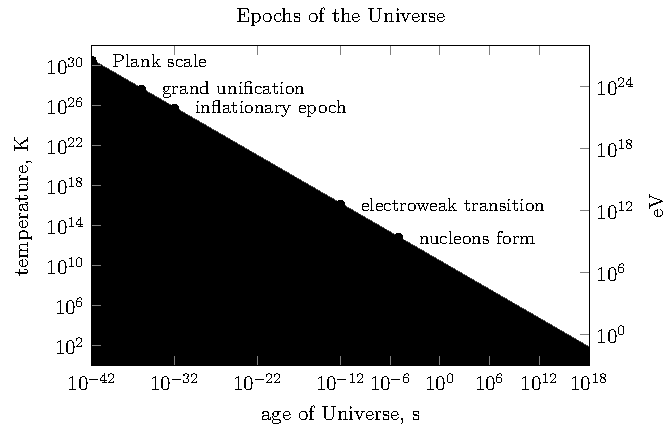
\includegraphics{diagrams/big-history.pdf}
	\caption{Temperature $T$ of the universe from the Big Bang to the present.}
\end{figure}

A few minutes after the beginning of time, when the universe cooled to $\sim 10^{10}\,\si{\K}$ during \emph{Big Bang nucleosynthesis} (BBN), protons and neutrons began to bind together to form light atomic nuclei.
The primary fusion reactions that occurred are:
\begin{align}
	\el{p + n} &\to \el{^2H} + γ
\\	\el{p + {}^2H} &\to \el{^3He} + γ
\\	\el{^2H + {}^2H} &\to \el{^3He + n, {}^3H + p}
\\	\el{^3He + {}^2H} &\to \el{^4He + p}
\\	&\ \vdots
\end{align}
Photons are involved in the production of deuterium $^2\el H$ and the lightest isotopes of helium, but not in the fusion of heavier nuclei.
An analysis of the reaction rates provides a relationship between the photon abundance $n_γ$ and the abundance of light nuclei (i.e., baryons, $n_B$).
A larger initial baryon--photon ratio $η = n_B/n_γ$ corresponds to more efficient production of deuterium and ultimately to a larger helium $^4\el{He}$ abundance in the present.
Relative element abundances in the present epoch constrain the value of the initial baryon--photon ratio to $η = (6.2 \pm 0.4) \times 10^{-10}$ \cite[§\,24.4]{ParticleDataGroup-review-2020}.


\begin{figure}
	\centering
	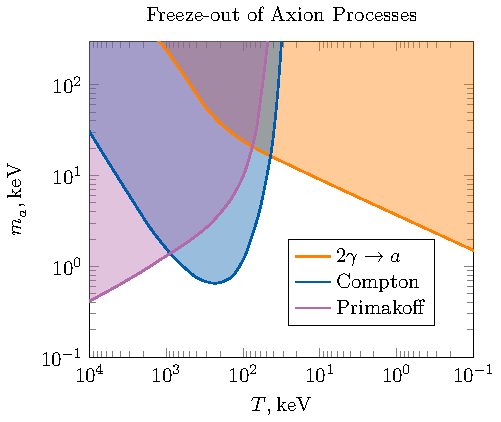
\includegraphics{diagrams/cosmo-freeze-out.pdf}
	\caption{
		Axion decoupling and recoupling with varying cosmological temperature, as in \cite{Cadamuro_2011}.
		The evolution of the universe progresses from left-to-right, in the direction of \emph{decreasing} temperature.
		Shaded regions indicate periods where each processes occurs spontaneously and axions are thermalised.
		Each horizontal line represents a possible timeline of axion freeze-out and recombination.
		The upper edge of the plot is the line $m_a = \SI{300}{\kilo\eV}$.
	}
	\label{fig:axion-freeze-out}
\end{figure}


Equipped with a cosmological model of axion interactions, Cadamuro \etal.\ solve the associated Boltzmann equation for the axion abundance $n_a$ over time as a function of mass $m_a$.
At later epochs, the axions eventually decay by $a \to 2γ$, increasing the entropy and abundance of photons in proportion to $n_a$ at late times.
This is measurable as an increase of the temperature of the cosmic microwave background (CMB), or equivalently, as a decrease in abundance of baryons and neutrinos relative to the CMB.
This can be compared to observation and used to limit the photon excess due to axion decay, in turn limiting $n_a$, which constrains the axion mass $m_a$.
Cadamuro \etal.\ find that the predicted deuterium abundance is reduced two standard deviations below its observed value for axion masses less than $\SI{300}{\kilo\eV}$, thus obtaining the limit
\begin{align}
	m_a \gtrsim \SI{300}{\kilo\eV}
	\label{eqn:cosmo-limit}
\end{align}
at $2σ = \SI{97}{\percent}$ confidence \cite{Cadamuro_2011}.
Axions within this bound decay into photons sufficiently quickly so as not to deviate the outcome of BBN from observation.
Such heavy axions are thermalised at all epochs, even purely hadronic axions which do not undergo Compton scattering (see figure~\ref{fig:axion-freeze-out}).
The limit \eqref{eqn:cosmo-limit} therefore applies to all axion types, and is far more restrictive than laboratory constraints.



\subsection{Constraints from Stellar Evolution}


Galaxies consist of \emph{globular clusters} (GCs), each typically consisting of between $10^5$ and $10^7$ stars.
A typical galaxy like our own hosts hundreds of GCs, each one a gravitationally self-contained island of stars.
The population of a GC can be partitioned into different branches by stage of stellar evolution, as in figure~\ref{fig:globular-cluster}.
Young stars exist in the main sequence and approach the \emph{red giant branch} (RGB) as they burn hydrogen fuel and produce helium.
Red giants approach the helium fusion phase as their cores become \el{He}-dense and \el{H}-depleted.
The ignition of \el{He}-fusion in late-stage red giants causes an immediate rise in temperature and rate of \el{He}-fusion, transitioning the star into a new equilibrium state in the \emph{horizontal branch} (HB) \cite[§\,3.2]{Irastorza_2018}.
The parameter $R \coloneqq N_\text{RGB}/N_\text{HB}$ is defined as the population ratio between the horizontal and red giant branches in a given GC, and is a useful observable for testing models of stellar evolution.

The alleged production of axions in stars has implications for stellar evolution.
Specifically, axion production via the Primakoff process $γ + A \to A + a$ in stellar plasma results in a hotter core temperature and faster burning of helium fuel in red giants.
This affects the relative durations of the RGB and HB stages.
The observed population of stars in each stage of the stellar sequence is statistically proportional to the stage's average lifetime, and thus the observable $R$ parameter measures relative stage lifetimes, $R = N_\text{RGB}/N_\text{HB} = T_\text{RGB}/T_\text{HB}$.
Thus, the axion--photon interaction strength may be constrained by comparing the predicted $R$-parameter to those observed in local GCs.
A recent survey \cite{Stellar-evolution-constraints_2015,Stellar-evolution-constraints_2020} of 39 of GCs reports the constraint $|g_{aγγ}| < \SI{6.5e-11}{\per\giga\eV}$ at \SI{95}{\percent} confidence \cite[§\,3.2]{Irastorza_2018}.
Stronger interacting axions cause horizontal branch stars to burn too quickly, reducing the $R$-parameter below the observed window.


\begin{figure}
	\centering
	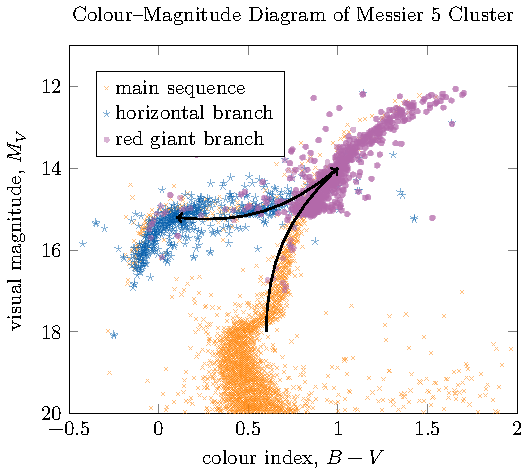
\includegraphics{diagrams/globular-cluster.pdf}
	\caption{An example colour-magnitude plot for the Messier 5 globular cluster, showing main branches of stellar evolution.
	The visual magnitude encodes luminosity (increasing upwards) and the colour index encodes surface temperature (increasing right-to-left).
	Stellar evolution flows in the direction of the arrows.
	}
	% \note{(Data from \cite{M5_CM_diagram}.)}}
	\label{fig:globular-cluster}
\end{figure}






\section{Conclusions and Outlook}

It is only a possibility that axions exist, and if it does, it remains elusively in the ever-shrinking non-excluded areas of parameter space.

\subsubsection{Axions and Dark Matter, Inflation and Baryogenesis}

